\documentclass[14pt]{beamer}
\usetheme{Warsaw}
\usecolortheme{beaver}
\usefonttheme{professionalfonts}

\input{../../preamble}
\usepackage{amscd,amsmath,amssymb,amsthm,graphicx}
\usepackage{paralist}
\usepackage{tabto}
\usepackage[normalem]{ulem}
\usepackage{tikz}
\usepackage{tkz-euclide}
\usetkzobj{all}
\newcommand{\dint}{\displaystyle\int}
\newcommand{\dlim}{\displaystyle\lim}
\newcommand{\dsum}{\displaystyle\sum}

% % % % % % % % % %
\title[Cal I S2015]{MATH 2554 (Calculus I)}
\subtitle{}
\author[Wheeler]{Dr. Ashley K. Wheeler}
\institute{University of Arkansas}
\date{\today}
\logo{}

% % %
\begin{document}
\maketitle

% % %
\begin{frame}
\frametitle{Table of Contents}
\tableofcontents
\end{frame}

% % % % % % % % % % Mon 13 Apr 2015

% % %
\begin{frame}
\section[Week 13]{Week 13: 13-17 April}
\frametitle{Monday 13 April (Week 13)}
\small
\begin{itemize}
\item Quiz \#12 In Class ($\oint 5.1$ and $\Sigma$ notation) Thurs 16 April, then Quiz \#13 ($\oint 4.8, 5.1, 5.2$) Take Home due Tues 20 Apr
\item \alert{Friday 17 April is the deadline to drop for a ``W" on your transcript}
\item Exam \#4 Friday 24 April
\end{itemize}
\end{frame}

% % %
\begin{frame}
\subsection[$\oint 5.1$ Approximating Area Under Curves]{$\oint 5.1$ Approximating Area Under Curves}
\frametitle{$\oint 5.1$ Approximating Area Under Curves}
\small
\begin{ex} Suppose you ride your bike at a constant velocity of 8 miles per hour for 1.5 hours.
\begin{itemize}
\item What is the velocity function that models this scenario?
\item What does the graph of the velocity function look like?
\item What is the position function for this scenario?
\item Where is the displacement (i.e., the distance you've traveled) represented when looking at the graph of the velocity function?
\end{itemize}
\end{ex}
\end{frame}

% % %
\begin{frame}
\small
In the previous example, the velocity was constant.  In most cases, this is not accurate (or possible).  How could we find displacement when the velocity is changing over an interval?

\bigskip

One strategy is to divide the time interval into a particular number of subintervals and approximate the velocity on each subinterval with a constant velocity.  Then for each subinterval, the displacement can be evaluate and summed.

\bigskip

Note:  This provides us with only an approximation, but with a larger number of subintervals, the approximation becomes more accurate.
\end{frame}

% % %
\begin{frame}
\frametitle{}
\footnotesize
\begin{ex} Suppose the velocity of an object moving along a line is given by $v(t)=\sqrt{10t}$ on the interval $1 \le t \le 7$.  Divide the time interval into $n=3$ subintervals, assuming the object moves at a constant velocity equal to the value of $v$ evaluated at the midpoint of the subinterval.  Estimate the displacement of the object on $[1,7]$.  Repeat for $n=6$ subintervals. \end{ex}

\vspace{-0.5pc}
\begin{center}
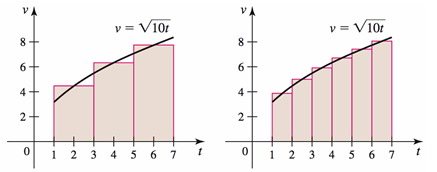
\includegraphics[scale=0.9]{Ch5Sect1_Exer10}
\end{center}
\end{frame}

% % %
\begin{frame}
\frametitle{\small Riemann Sums}
\small
%The more subintervals you divide your time interval into, the more accurate your approximation of displacement will be (see Example 1 on pp.\ 307--308).

%We now examine a method for approximating areas under curves.

Consider a function $f$ over the interval $[a,b]$.  Divide $[a,b]$ into $n$ subintervals of equal length:
\[[x_0,x_1], [x_1,x_2], \dots, [x_{n-1},x_n]\]
with $x_0=a$ and $x_n=b$.  The length of each subinterval is denoted
\[\Delta x = \frac{b-a}{n}.\]
\end{frame}

% % %
\begin{frame}
\small
In each subinterval $[x_{k-1}, x_k]$, we can choose any point $\overline{x}_k$ and create a rectangle with a height of $f(\overline{x}_k)$.
The area of the rectangle is the product of its height and base, or $f(\overline{x}_k)\Delta x$.

\vspace{1pc}
Doing this for each subinterval, and then summing each rectangle's area, produces an approximation of the overall area.  This approximation is called a {\bf Riemann sum}
\[R=f(\overline{x}_1)\Delta x + f(\overline{x}_2)\Delta x + \cdots + f(\overline{x}_n)\Delta x.\]
\end{frame}

% % %
\begin{frame}
\footnotesize
Note:  We let $k$ vary from $1$ to $n$, and we always have 
\[x_{k-1}\leq \overline x_k\leq x_k.\]  
We usually choose $\overline{x}_k$ so that it is consistent across all the subintervals.  The most common ways to do this are with {\bf left Riemann sums}, {\bf right Riemann sums}, and {\bf midpoint Riemann sums}.  (See Figures 5.9--5.11 on p.\ 310--312 for pictures of these sums.)

\vspace{1pc}
Let $R=f(\overline{x}_1)\Delta x + f(\overline{x}_2)\Delta x + \cdots + f(\overline{x}_n)\Delta x$.
\begin{itemize}
\item[1.] $R$ is a {\bf left Riemann sum} when we choose $\overline x_k=x_{k-1}$ for each $k$.  
\item[2.] $R$ is a {\bf right Riemann sum} when we choose $\overline x_k=x_k$ for each $k$.
\item[3.] $R$ is a {\bf midpoint Riemann sum} when we take $\overline x_k$ to be the midpoint between $x_{k-1}$ and $x_k$, for each $k$.  
\end{itemize}
\end{frame}

% % %
\begin{frame}
\frametitle{\small Sigma Notation}
\footnotesize
Riemann sums become more accurate when we make $n$ (the number of rectangles) bigger.  However, writing it down becomes a pain.  Sigma notation gives a shorthand.  

%Recall how sigma notation works:  $\displaystyle\sum_{n=1}^5 n^2$ means to sum all integer values from the lowest limit ($n=1$) to the highest limit ($n=5$) in the summand $n^2$.  So 
\begin{ex} \[\dsum_{n=1}^5 n^2 = 1^2+2^2+3^2+4^2+5^2=55.\] \end{ex}

\begin{exe} Evaluate $\displaystyle\sum_{k=0}^3 (2k-1)$. \end{exe}
\end{frame}

% % %
\begin{frame}
\frametitle{\small $\Sigma$-Shortcuts}
\footnotesize
($n$ is always a positive integer)
\begin{align*}
\dsum_{k=1}^n c & = cn \text{ (where $c$ is a constant)} \\[0.5pc]
\dsum_{k=1}^n k &= \dfrac{n(n+1)}{2} \\[0.5pc]
\dsum_{k=1}^n k^2 &= \dfrac{n(n+1)(2n+1)}{6} \\[0.5pc]
\dsum_{k=1}^n k^3 &= \dfrac{n^2(n+1)^2}{4}
\end{align*}
\end{frame}

% % %
\begin{frame}
\frametitle{\small Riemann Sums Using Sigma Notation}
\small
Now using sigma notation, we can write the Riemann sum in a much more compact form:
\begin{align*}
R &= f(\overline{x}_1)\Delta x + f(\overline{x}_2)\Delta x + \cdots + f(\overline{x}_n)\Delta x \\[0.5pc]
 &= \dsum_{k=1}^n f(\overline{x}_k) \Delta x.
 \end{align*}

%To write the left, right, and midpoint Riemann sums in sigma notation, we need to know the point $\overline{x}_k$.
\end{frame}

% % %
\begin{frame}
\frametitle{\small Left, Right, and Midpoint Riemann Sums in Sigma Notation}
\footnotesize
Suppose $f$ is defined on a closed interval $[a,b]$ which is divided into $n$ subintervals of equal length $\Delta x$.  As before, let $\overline{x}_k$ denote a point in the $k$th subinterval $[x_{k-1},x_k]$, for $k=1,2,\dots,n$.  Also, notice that $x_0=a$ and $x_n=b$. 

\begin{itemize}
\item[1.] $\dsum_{k=1}^n f(\alert{a+(k-1)\Delta x}) \Delta x$ gives a left Riemann sum.
\item[2.] $\dsum_{k=1}^n f(\alert{a+k\Delta x}) \Delta x$ gives a right Riemann sum.
\item[3.] $\dsum_{k=1}^n f(\alert{a+\left(k-\dfrac{1}{2}\right)\Delta x}) \Delta x$ gives a midpoint Riemann sum.
\end{itemize}
\end{frame}

% % % % % % % % % % Wed 15 Apr 2015

% % %
\begin{frame}
\frametitle{Wednesday 15 April (Week 13)}
\small
\begin{itemize}
\item Quiz \#12 In Class ($\oint 5.1$ and $\Sigma$ notation) Thurs 16 April, then Quiz \#13 ($\oint 4.8, 5.1, 5.2$) Take Home due Tues 20 Apr
\item \alert{Friday 17 April is the deadline to drop for a ``W" on your transcript}
\item Exam \#4 Friday 24 April
\end{itemize}
\end{frame}

% % %
\begin{frame}%[t]
\frametitle{}
\begin{exe} Use sigma notation to write the left, right, and midpoint Riemann sums for the function $f(x)=x^2$ on the interval $[1,5]$ given that $n=4$.

\vspace{1pc}
Based on these approximations, estimate the area bounded by the graph of $f(x)$ over $[1,5]$.
\end{exe}
\end{frame}

% % %
\begin{frame}
\frametitle{HW from Section 5.1}
Do problems 9, 11, 15--23 odd, 31, 33, 53--57 all (pp.\ 315--320 in textbook)
\end{frame}

% % % % % % % % % % Fri 17 Apr 2015

% % %
\begin{frame}
\frametitle{Friday 17 April (Week 13)}
\small
\begin{itemize}
\item Quiz \#14 Tues 21 April in class ($\oint 5.3-5.4$)
\item Exam 4 Friday 24 April
\item Quiz \#15 28 April in class ($\oint 5.5$)
\end{itemize}
\end{frame}

% % %
\begin{frame}
\subsection[$\oint 5.2$ Definite Integrals]{$\oint 5.2$ Definite Integrals}
\frametitle{$\oint 5.2$ Definite Integrals}
\small
In 5.1, we saw how we can use Riemann sums to approximate the area under a curve.  However, the curves we worked with were all non-negative.

\vspace{1pc}
What happens when the curve is negative?
\begin{ex} Let $f(x)=8-2x^2$ over the interval $[0,4]$.  Use a left, right, and midpoint Riemann sum with $n=4$ to approximate the area under the curve. \end{ex}
\end{frame}

% % %
\begin{frame}
\frametitle{}
\footnotesize
In the previous ex., the areas where $f$ was positive provided positive contributions to the area, while areas where $f$ was negative provided negative contributions.  The difference between positive and negative contributions is called the {\bf net area}.

\vspace{1pc}
\begin{dfn} Consider the region $R$ bounded by the graph of a continuous function $f$ and the $x$-axis between $x=a$ and $x=b$.  The {\bf net area} of $R$ is the sum of the areas of the parts of $R$ that lie above the $x$-axis minus the sum of the areas of the parts of $R$ that lie below the $x$-axis on $[a,b]$. \end{dfn}
\end{frame}

% % %
\begin{frame}
\frametitle{\small Definite Integral}
\small
The Riemann sums give approximations for the area under the curve.  To make these approximations more and more accurate, we divide the region into more and more subintervals.

\bigskip

To make these approximations exact, we allow the number of subintervals $n \to \infty$, thereby allowing the length of the subintervals $\Delta x \to 0$.  In terms of limits:
$$\text{Net Area}=\lim_{n \to \infty} \sum_{k=1}^n f(\overline{x}_k) \Delta x.$$
\end{frame}

% % %
\begin{frame}
\frametitle{\small General Riemann Sums}
\footnotesize
Suppose $[x_0,x_1], [x_1,x_2], \dots, [x_{n-1},x_n]$ are subintervals of $[a,b]$ with $a=x_0 < x_1 < x_2 < \cdots < x_{n-1} < x_n=b$.

\bigskip

Let $\Delta x_k$ be the length of the subinterval $[x_{k-1},x_k]$ and let $\overline{x}_k$ be any point in $[x_{k-1},x_k]$ for $k=1,2,\dots,n$.

\bigskip

If $f$ is defined on $[a,b]$, then the sum
\[\sum_{k=1}^n f(\overline{x}_k) \Delta x_{\alert k} = f(\overline{x}_1)\Delta x_{\alert 1} + f(\overline{x}_2)\Delta x_{\alert 2} + \dots + f(\overline{x}_n)\Delta x_{\alert n}\]
is called a {\bf general Riemann sum for $\boldsymbol{f}$ on $\boldsymbol{[a,b]}$}.

\bigskip

(In this definition, the lengths of the subintervals do not have to be equal.)
\end{frame}

% % %
\begin{frame}
\frametitle{\small The {\it Definite} Integral}
\footnotesize
As $n \to \infty$, all of the $\Delta x_k \to 0$, even the largest of these.  Let $\Delta$ be the largest of the $\Delta x_k$'s.  The we look for 
\[\displaystyle\lim_{\Delta \to 0} \dsum_{k=1}^n f(\overline{x}_k) \Delta x_k.\] 

\vspace{-0.5pc}
\begin{dfn} A function $f$ defined on $[a,b]$ is {\bf integrable} means $\displaystyle\lim_{\Delta  \to 0} \sum_{k=1}^n f(\overline{x}_k) \Delta x_k$ exists -- over {\it all} partitions of $[a,b]$ and {\it all} choices of $\overline{x}_k$ on a partition.  This limit is the {\bf definite integral of $\boldsymbol{f}$ from $\boldsymbol{a}$ to $\boldsymbol{b}$}, which we write
\[\int_a^b f(x)\ dx = \lim_{\Delta  \to 0} \sum_{k=1}^n f(\overline{x}_k) \Delta x_k.\]
\end{dfn}
\end{frame}

% % %
\begin{frame}
\frametitle{\small Evaluating Definite Integrals}
\footnotesize
\begin{thm}
If $f$ is continuous on $[a,b]$ or bounded on $[a,b]$ with a finite number of discontinuities, then $f$ is integrable on $[a,b]$.
\end{thm}

\bigskip

See Figure 5.23, p.\ 325, for an example of a noncontinuous function that is integrable.

\bigskip

Knowing the limit of a Riemann sum, we can now translate that to a definite integral.

\begin{ex}$\displaystyle\lim_{\Delta  \to 0} \sum_{k=1}^n (4\overline{x}_k - 3)\Delta x_k$ on $[-1,4] \iff \dint_{-1}^4 (4x-3)\ dx.$ \end{ex}
\end{frame}

% % %
\begin{frame}%[t]
\frametitle{}
\small
\begin{exe} Using geometry, evaluate $\dint_1^2 (4x-3)\ dx.$ 

\bigskip

(Hint:  The area of a trapezoid is $\dfrac{h(a+b)}{2}$, where $h$ is the height of the trapezoid and $a$ and $b$ are the lengths of the two parallel bases.)
\end{exe}
\end{frame}

% % %
\begin{frame}
\frametitle{}
\footnotesize
\begin{exe} Using the picture below, evaluate the following definite integrals:
\[\text{1.\ } \int_0^a f(x)\ dx \qquad \text{2.\ } \int_0^b f(x)\ dx \qquad \text{3.\ } \int_0^c f(x)\ dx \qquad \text{4.\ } \int_a^c f(x)\ dx\]

\begin{center}
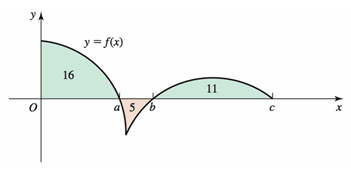
\includegraphics[scale=0.9]{Ch5Sect2_Exer31}
\end{center}
\end{exe}
\end{frame}

% % %
\begin{frame}
\frametitle{\small Properties of Integrals}
\footnotesize
\begin{itemize}
\item[1.] (Reversing Limits) $\dint_b^a f(x)\ dx = -\dint_a^b f(x)\ dx$

\vspace{0.75pc}
\item[2.] (Identical Limits) $\dint_a^a f(x)\ dx = 0$

\vspace{0.75pc}
\item[3.] (Integral of a Sum) 

$\dint_a^b (f(x)+g(x))\ dx = \dint_a^b f(x)\ dx + \dint_a^b g(x)\ dx$

\vspace{0.75pc}
\item[4.] (Constants in Integrals) $\dint_a^b cf(x)\ dx = c \dint_a^b f(x)\ dx$
\end{itemize}
\end{frame}

% % %
\begin{frame}
\frametitle{\small Properties of Integrals, cont.}
\footnotesize
\begin{itemize}

\item[5.] (Integrals over Subintervals) If $c$ lies between $a$ and $b$, then
$$\dint_a^b f(x)\ dx = \dint_a^c f(x)\ dx + \dint_c^b f(x)\ dx.$$

\item[6.] (Integrals of Absolute Values) The function $|f|$ is integrable on $[a,b]$ and $\dint_a^b |f(x)|\ dx$ is the sum of the areas of regions bounded by the graph of $f$ and the $x$-axis on $[a,b]$.  (See Figure 5.31 on p.\ 329) \alert{(This is the total area, no negative signs.)}
\end{itemize}
\end{frame}

% % %
\begin{frame}%[t]
\frametitle{}
\small
\begin{exe} If 
\[\dint_2^4 f(x)\ dx = 3\quad\text{ and }\quad \dint_4^6 f(x)\ dx = -2,\] 
then compute 
\[\dint_2^6 f(x)\ dx.\] \end{exe}
\end{frame}

% % %
\begin{frame}
\frametitle{HW from Section 5.2}
Do problems 11--29 odd, 35--44 all, 65 (pp.\ 331--333 in textbook)
\end{frame}

% % %
\begin{frame}
\subsection[$\oint 5.3$ Fundamental Theorem of Calculus]{$\oint 5.3$ Fundamental Theorem of Calculus}
\frametitle{$\oint 5.3$ Fundamental Theorem of Calculus}
\small
Using Riemann sums to evaluate definite integrals is usually neither efficient nor practical.  We will develop methods to evaluate integrals and also tie together the concepts of differentiation and integration.  
\end{frame}

% % %
\begin{frame}
\frametitle{\small Area Functions}
\footnotesize
Let $y=f(t)$ be a continuous function which is defined for all $t \ge a$, where $a$ is a fixed number.  The area function for $f$ with left endpoint at $a$ is given by 

\vspace{-1.5pc}
\[A(x)=\dint_a^x f(t)\ dt.\]  

\vspace{-1.8pc}
\begin{center}
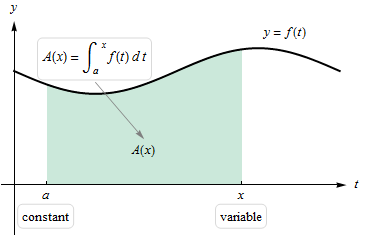
\includegraphics[scale=0.55]{Fig5_32}
\end{center}

\vspace{-1.5pc}
This gives the net area of the region between the graph of $f$ and the $t$-axis between the points $t=a$ and $t=x$.  (See Figure 5.33 on p.\ 335 for pictures of the area function in action.) 
\end{frame}

% % %
\begin{frame}
\frametitle{}
\footnotesize
\begin{exe} The graph of $f$ is shown below.  Let 

\vspace{-0.75pc}
\[A(x)=\dint_0^x f(t)\ dt\quad\text{ and }\quad F(x)=\dint_2^x f(t)\ dt\] 

\vspace{-0.25pc}
be two area functions for $f$.  Compute $A(2), F(5), A(5), F(8)$.

\vspace{-0.65pc}
\begin{center}
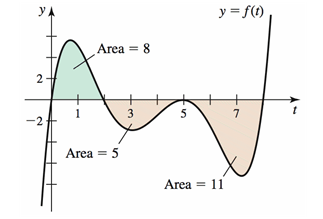
\includegraphics[scale=0.85]{Ch5Sect3_Exer12}
\end{center}
\end{exe}
\end{frame}

% % %
\begin{frame}
\frametitle{\small The Fundamental Theorem of Calculus (Part 1)}
\footnotesize
\begin{thm}[FTOC I] If $f$ is continuous on $[a,b]$, then the area function 
\[A(x)=\dint_a^x f(t)\ dt\] 
for $a \le x \le b$ is continuous on $[a,b]$ and differentiable on $(a,b)$.  The area function satisfies $A^{\prime}(x)=f(x)$; or equivalently, 
\[A^{\prime}(x)=\frac{d}{dx} \dint_a^x f(t)\ dt = f(x)\]
which means that the area function of $f$ is an antiderivative of $f$.
\end{thm}
\end{frame}

% % %
\begin{frame}
\frametitle{\small The Fundamental Theorem of Calculus (Part 2)}
\small
Since $A$ is an antiderivative of $f$, we now have a way to evaluate definite integrals and find areas under curves.

\begin{thm}[FTOC II] If $f$ is continuous on $[a,b]$ and $F$ is any antiderivative of $f$, then
\[\int_a^b f(x)\ dx = F(b)-F(a).\]
\end{thm}

\vspace{1pc}
We use the notation $F(x) \vert_a^b = F(b)-F(a)$.
\end{frame}

% % %
\begin{frame}
\frametitle{\small Overview of FTOC}
\small
In essence, to evaluate an integral, we
\begin{itemize}
\item Find any antiderivative of $f$, and call if $F$.
\item Compute $F(b)-F(a)$, the difference in the values of $F$ between the upper and lower limits of integration.
\end{itemize}

The two parts of the FTOC illustrate the inverse relationship between differentiation and integration -- the integral ``undoes'' the derivative.
\end{frame}

% % %
\begin{frame}%[t]
\frametitle{}
\small
\begin{exe}
\begin{itemize}
\item Use Part 1 of the FTOC to simplify $\dfrac{d}{dx} \dint_x^{10} \dfrac{dz}{z^2+1}$.

\vspace{0.75pc}
\item Use Part 2 of the FTOC to evaluate $\dint_0^{\pi} (1-\sin x)\ dx.$

\vspace{0.75pc}
\item Compute $\dint_1^y h^{\prime}(p)\ dp$.
\end{itemize}
\end{exe}
\end{frame}

% % %
\begin{frame}
\frametitle{HW from Section 5.3}  
Do problems 11--17 all, 19--39 odd, 45--57 odd (pp.\ 346--347 in textbook)
\end{frame}


\begin{comment}
\end{comment}

\end{document}